\chapter{Results} \label{chap:experimental-results}
Using the automated measurement and post-processing workflow for off-axis EH detailed in \cref{ssec:off-axis-EH-experimental-setup} as well as FEM simulations using the \emph{ONELAB} and \emph{nextnano} software packages described in \cref{sec:numerical-modeling}, the following chapter details the results obtained from both experimental measurements and simulations and compares them in the context of quantitative agreement.
\section{Coplanar Capacitor} \label{sec:experimental-results-coplanar-capacitor}
The ubiquitous coplanar capacitor, whose preparation is described in detail in \cref{ssec:specimen-preparation-capacitor}, was used as a reference specimen due to its well known geometry and electrostatic behavior.
\subsection{Off-Axis Electron Holography} \label{ssec:experimental-results-capacitor-EH}
For the first measurement series, three object holograms and two empty holograms were recorded for an exposure time of $T_{\mathit{exp}} = \SI{5}{\second}$ each using a filament voltage of $U_f \approx \SI{75}{\volt}$. The external electrical bias $U_{\mathit{ext}}$ was chosen from $\SIrange{-1.5}{1.5}{\volt}$ in increments of $\SI{0.3}{\volt}$ as well as $\SIrange{-1.0}{1.0}{\volt}$ in increments of $\SI{0.5}{\volt}$. The acquired holograms were then reconstructed using the upper sideband where a 14\textsuperscript{th} degree Butterworth filter with a cut-off frequency of $1/\SI[per-mode=power]{11.4}{\per\nm}$, yielding a spatial resolution of approximately $\SI{20}{\nm}$ \cite{Lehmann2002,Lichte2008}, was applied.
\newpage
For an external bias voltage of $U_{\mathit{ext}} = \SI{1}{\volt}$ applied to the upper contact, with the lower contact grounded, the reconstructed amplitude $A$ (normalized to $1$) and its line profile $A\left(x\right)$ (illustrated by a blue rectangle with an arrow indicating the direction) show a constant behavior between the capacitor plates with slight modulations at the edges due to Fresnel fringes (\cref{fig:capacitor-off-axis-EH-linescans}a). The reconstructed phase $\varphi$ on the other hand is constrained to an interval of $\interval{-\pi}{\pi}$, where its line profile $\varphi\left(x\right)$ in the same region as \cref{fig:capacitor-off-axis-EH-linescans}a) shows a linear trend between the capacitor plates and noise within them (\cref{fig:capacitor-off-axis-EH-linescans}b).
\begin{figure}[H]
	\centering
	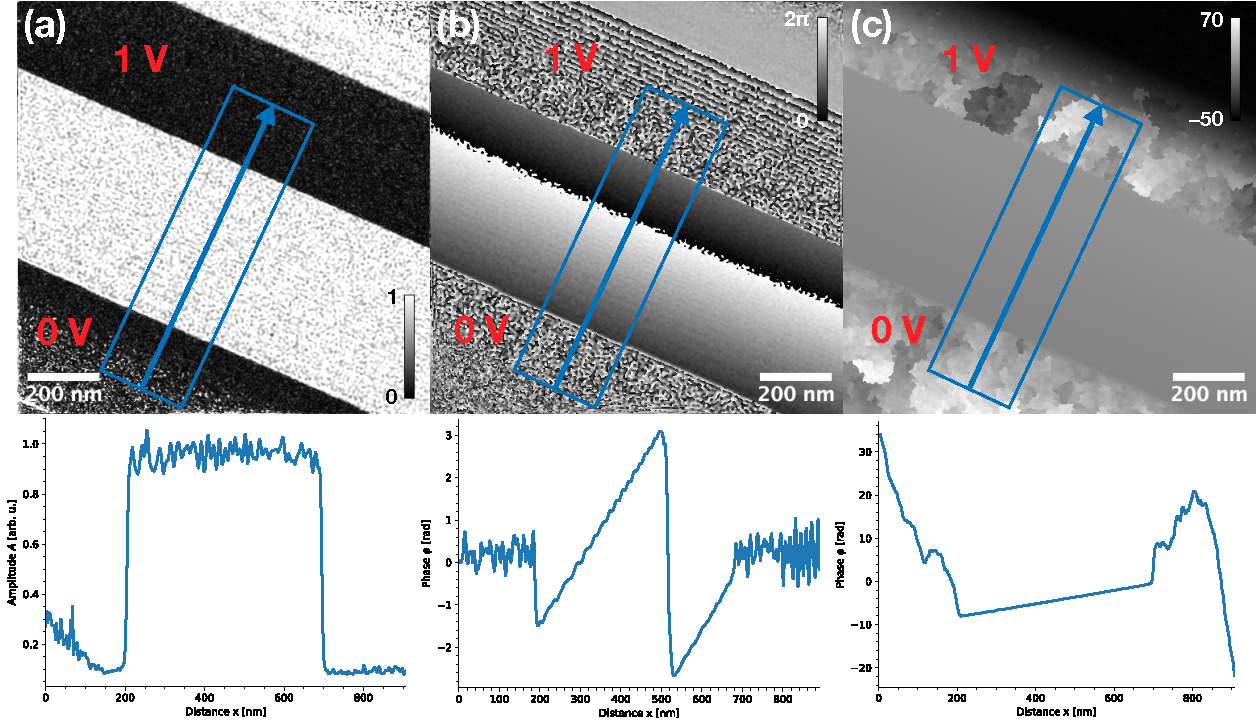
\includegraphics[width=\textwidth]{Figures/Results/Capacitor/Holography/capacitor-off-axis-EH-linescans.pdf}
	\caption{Electron holography for a coplanar capacitor biased with $U_{\mathit{ext}} = \SI{1}{\volt}$ with (a) the reconstructed amplitude and its corresponding line profile $A\left(x\right)$, (b) the reconstructed phase and its corresponding $2\pi$-wrapped line profile $\varphi\left(x\right)$ and (c) the same reconstructed phase and its line profile unwrapped.}
	\label{fig:capacitor-off-axis-EH-linescans}
\end{figure}
Unwrapping the phase image yields the same linear trend with the $2\pi$ phase jumps removed (\cref{fig:capacitor-off-axis-EH-linescans}c), while the unwrapping algorithm produces undefined behavior for the contacts consisting primarily of noise and arbitrary phase offsets for non-contiguous areas (e.\,g.\ reference window).
\newpage
Comparing the phase image for an applied external bias of $U_{\mathit{ext}} = \SI{1}{\volt}$ with the phase image for a short-circuited setup (i.\,e.\ $U_{\mathit{ext}} = \SI{0}{\volt}$), the vacuum region between the electrodes exhibits a characteristic gradient perpendicular to the surfaces of the capacitor plates (\cref{fig:capacitor-off-axis-EH-slope}a). Furthermore, varying the applied external bias between $U_{\mathit{ext}} = \SI{-1.5}{\volt}$ and $U_{\mathit{ext}} = \SI{1.5}{\volt}$ and normalizing the phase slopes $\dv*{\varphi}{x}$ calculated inside the vacuum region (illustrated by a blue rectangle with an arrow indicating the direction) to the phase slope at $U_{\mathit{ext}} = \SI{0}{\volt}$ displays the expected linear proportionality between the phase (and therefore the electrostatic potential) and the applied external voltage (\cref{fig:capacitor-off-axis-EH-slope}b).
\begin{figure}[H]
	\centering
	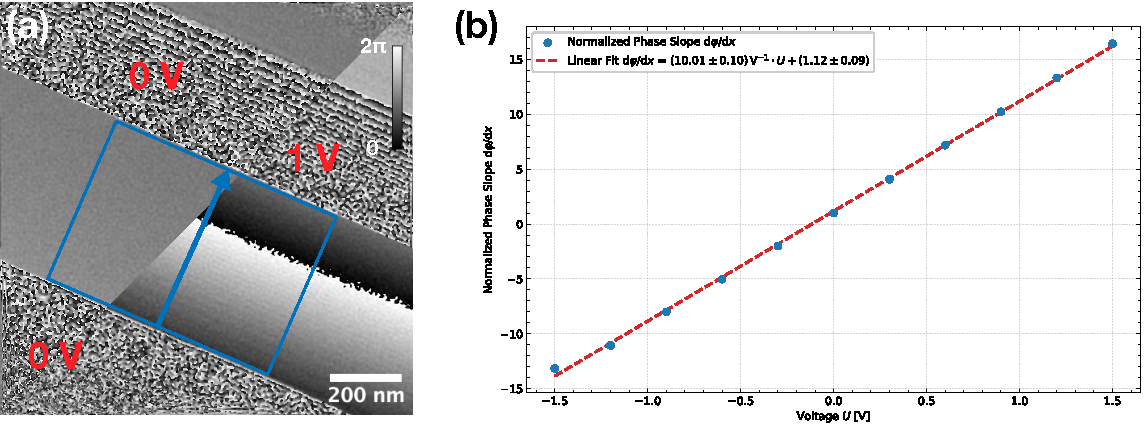
\includegraphics[width=\textwidth]{Figures/Results/Capacitor/Holography/capacitor-off-axis-EH-slope.pdf}
	\caption{Electron holography for a coplanar capacitor (a) biased with $U_{\mathit{ext}} = \SI{0}{\volt}$ and $U_{\mathit{ext}} = \SI{1}{\volt}$ and (b) the phase slopes $\dv*{\varphi}{x}$ for different external biasing voltages normalized to the phase slope at $U_{\mathit{ext}} = \SI{0}{\volt}$.}
	\label{fig:capacitor-off-axis-EH-slope}
\end{figure}
These observations not only illustrate the excepted linear slope of the electrostatic potential inside a vacuum region between two capacitor plates, which is linearly proportional to the applied external bias, but also show that EH is a suitable technique for the measurement of pure phase objects (as is the case here) where there is no apparent amplitude modulation.
\newpage
\subsection{Finite Element Method Simulation} \label{ssec:experimental-results-capacitor-FEM-simulation}
A comparable coplanar capacitor is modeled using the \emph{ONELAB} software package (\cref{fig:capacitor-FEM-EH-linescan-comparison}), whose exact geometric layout (\cref{fig:specimen-capacitor-layout}) is described in detail in \cref{ssec:2d-modeling-specimen}.
\begin{figure}[H]
	\centering
	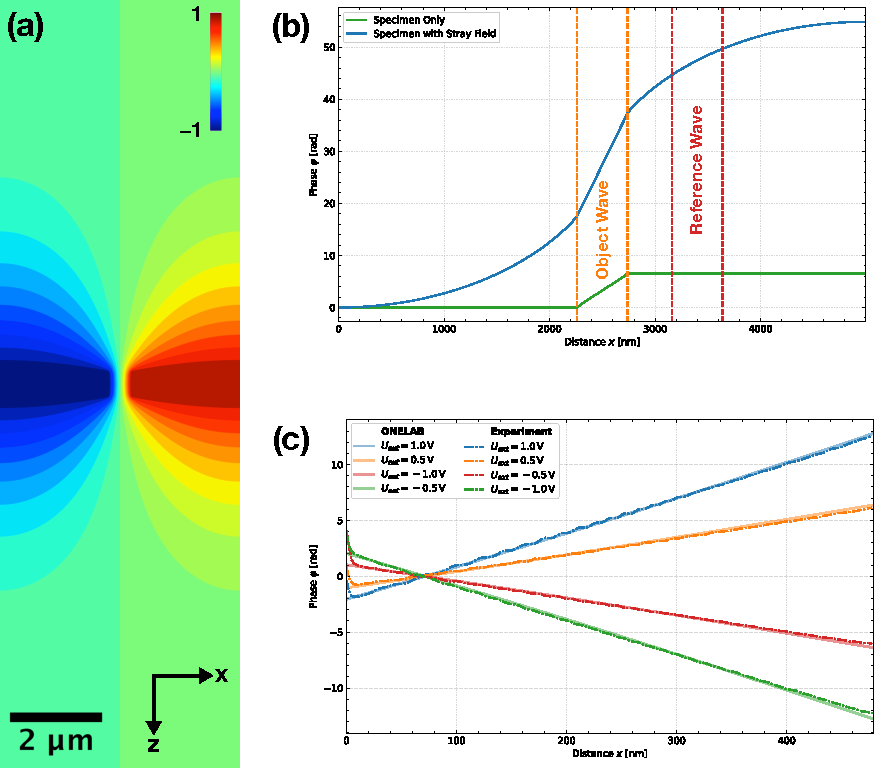
\includegraphics[width=\textwidth]{Figures/Results/Capacitor/Simulations/capacitor-FEM-EH-linescan-comparison.pdf}
	\caption{FEM simulation of the coplanar capacitor biased with $U_{\mathit{ext}} = \SI{1}{\volt}$ where (a) the 2D~electrostatic potential $\phi$ yields (b) the phase $\varphi$ through projection, (c) which is compared with the above detailed experimentally acquired holograms for different applied bias voltages.}
	\label{fig:capacitor-FEM-EH-linescan-comparison}
\end{figure}
The 2D~electrostatic potential $\phi$ obtained through this method shows that, while the contacts exhibit a constant potential of $\pm U_{\mathit{ext}}$, respectively, the stray field extents deep into the vacuum region above and below the capacitor, only approaching zero after several $\si{\um}$ (\cref{fig:capacitor-FEM-EH-linescan-comparison}a). This behavior is especially apparent when calculating the phase $\varphi$ through a projection (without any weighting applied to the different specimen regions), where the specimen (i.\,e.\ the capacitor itself) only contributes a small parts to the overall phase (approximately 8\% of the maximum phase shift), which is predominantly made up of the stray field contribution (\cref{fig:capacitor-FEM-EH-linescan-comparison}b, with both phases offset to zero through subtraction by the first value). Additionally, by defining the object wave $\varphi_{\mathit{obj}}$ to correspond to the vacuum region between the contacts (\cref{fig:capacitor-FEM-EH-linescan-comparison}b, indicated by the dashed orange lines) and the reference wave $\varphi_{\mathit{ref}}$ to a region of the same size offset $\SI{800}{\nm}$ to the right (\cref{fig:capacitor-FEM-EH-linescan-comparison}b, indicated by the dashed red lines), comparisons to the above experimentally acquired phases are made (\cref{fig:capacitor-FEM-EH-linescan-comparison}c).

Here, it is evident that for all external bias voltages $U_{\mathit{ext}}$, ranging from $\SIrange{-1.0}{1.0}{\volt}$ in increments of $\SI{0.5}{\volt}$, the simulated phases are in excellent agreement with the experimental phases acquired through off-axis EH.\footnote{Since the simulated coplanar capacitor was electrically biased by applying $\pm U_{\mathit{ext}}$ at the contacts, while the experimentally measured capacitor was grounded at one of the contacts, a scaling factor of $2$ has been applied when calculating the phase through projection.}

Through the comparison with 2D~simulations of the electrostatic potential, it is evident that FEM simulations are in excellent agreement with real-world measurements and are able to reliably describe the behavior of simple specimens. Furthermore, by separating the projected electrostatic potential into a specimen and stray field region, it is apparent that the specimen region of the coplanar capacitor only contributes a small part to the overall phase, necessitating a model which takes these effects into account.
\section[\texorpdfstring{$p$-$p^+$-$n^+$}{\textit{p}-\textit{p}\textsuperscript{+}-\textit{n}\textsuperscript{+}}-Junction]{$\boldsymbol{p}$-$\boldsymbol{p^+}$-$\boldsymbol{n^+}$-Junction}
The previous \cref{sec:experimental-results-coplanar-capacitor} successfully demonstrated the reliability of off-axis EH by analyzing the electrostatic behavior exhibited by a coplanar capacitor, which served as a well-understood reference specimen. This section shifts the focus towards the investigation of real semiconductor nanostructures, where a $p$-$p^+$-$n^+$-junction, whose preparation is described in detail in \cref{ssec:specimen-preparation-pn-junction}, serves as an exemplary specimen.
\subsection{Off-Axis Electron Holography} \label{ssec:experimental-results-ppn-junction-off-axis-EH}
The measurement series for the $p$-$p^+$-$n^+$-junction consisted of three object holograms and two empty holograms with an exposure time of $T_{\mathit{exp}} = \SI{5}{\second}$ each. The filament voltage was set to $U_f \approx \SI{69}{\volt}$ and the external electrical bias $U_{\mathit{ext}}$ was chosen from $\SIrange{0.0}{3.0}{\volt}$ in increments of $\SI{0.5}{\volt}$. Similar to the above described coplanar capacitor, the acquired holograms were reconstructed by applying a 14\textsuperscript{th} degree Butterworth filter with a cut-off frequency of $1/\SI[per-mode=power]{11.4}{\per\nm}$, whereas in this case the lower sideband was used.
\newpage
The diode was contacted with an external bias $U_{\mathit{ext}}$ at the $n^+$-doped region, whereas the $p$-doped region was grounded. By applying an external bias of $U_{\mathit{ext}} = \SI{2}{\volt}$ (i.\,e.\ reverse bias), the reconstructed amplitude $A$ exhibits a constant line profile $A\left(x\right)$ (illustrated by a blue rectangle with an arrow indicating the direction) across the junction (\cref{fig:pn-junction-off-axis-EH-linescans}a), similar to the above described coplanar capacitor. As is the case with the coplanar capacitor, the reconstructed phase $\varphi$ (with a phase wedge applied in the $p$-doped region) is constrained to an interval of $\interval{-\pi}{\pi}$, with its line profile $\varphi\left(x\right)$ displaying a characteristic phase jump caused by the built up of a potential barrier at the depletion region (\cref{fig:pn-junction-off-axis-EH-linescans}b).
\begin{figure}[H]
	\centering
	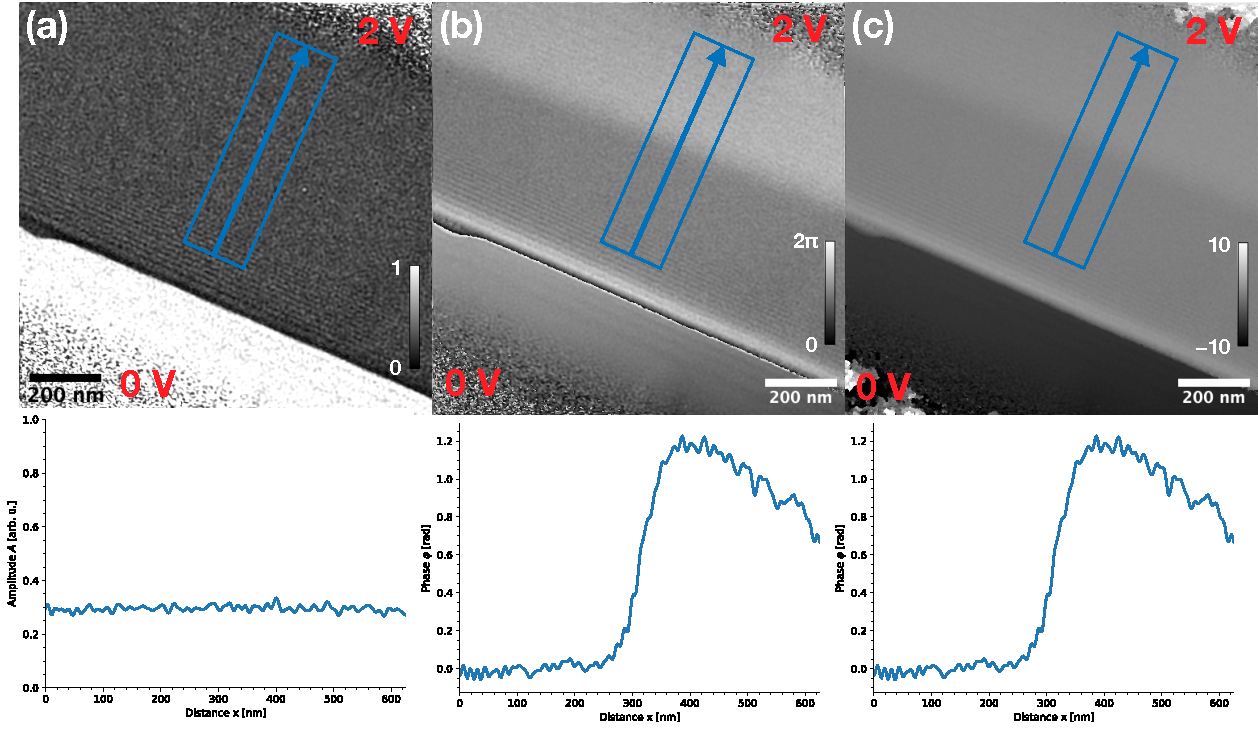
\includegraphics[width=\textwidth]{Figures/Results/pn-Junction/Holography/pn-junction-off-axis-EH-linescans.pdf}
	\caption{Electron holography for a $p$-$p^+$-$n^+$-junction reverse biased with $U_{\mathit{ext}} = \SI{2}{\volt}$ with (a) the reconstructed amplitude and its corresponding line profile $A\left(x\right)$, (b) the reconstructed phase (with a phase wedge applied in the $p$-doped region) and its corresponding $2\pi$-wrapped line profile $\varphi\left(x\right)$ and (c) the same reconstructed phase and its line profile unwrapped.}
	\label{fig:pn-junction-off-axis-EH-linescans}
\end{figure}
Unwrapping the phase image reveals an identical line profile across the junction due to the measured phase jump being smaller than $2\pi$ (\cref{fig:pn-junction-off-axis-EH-linescans}c), while unwrapping algorithm once again produces undefined behavior towards the contacts of the specimen.
\newpage
By comparing the phases images for an applied external bias of $U_{\mathit{ext}} = \SI{0}{\volt}$ and $U_{\mathit{ext}} = \SI{3}{\volt}$, only a moderate difference in the phase jump in reverse bias condition is observed (i.\,e.\ smaller than $2\pi$), indicating an abnormal switching behavior (\cref{fig:pn-junction-off-axis-EH-phase-jump}a). By comparing the phase jumps $\Delta \varphi\left(x\right)$ across the junction (illustrated by a blue rectangle with an arrow indicating the direction) for the different external bias voltages (after unwrapping and modulating each phase image by a phase wedge), the phase jumps, nonetheless, qualitatively demonstrate the expected proportionality to the externally applied voltage (\cref{fig:pn-junction-off-axis-EH-phase-jump}b).
\begin{figure}[H]
	\centering
	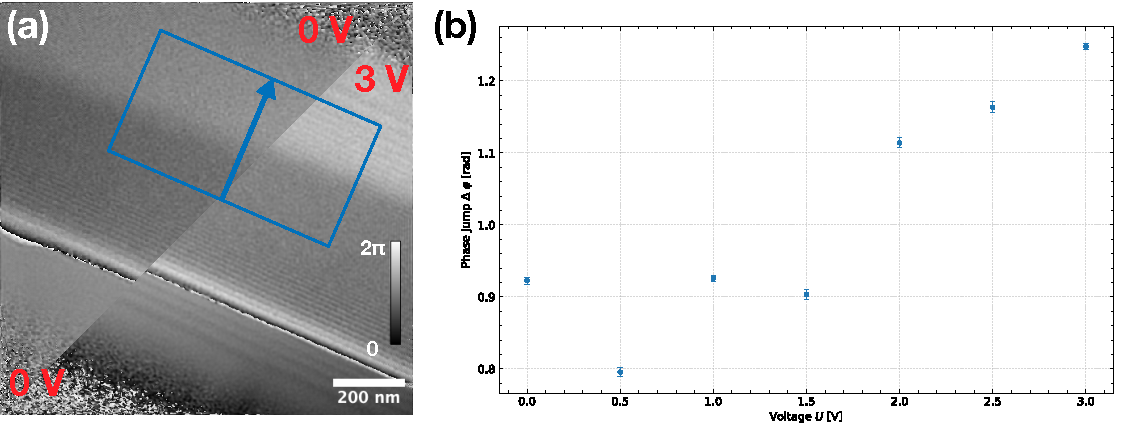
\includegraphics[width=\textwidth]{Figures/Results/pn-Junction/Holography/pn-junction-off-axis-EH-phase-jump.pdf}
	\caption{Electron holography for a $p$-$p^+$-$n^+$-junction (a) $U_{\mathit{ext}} = \SI{0}{\volt}$ and $U_{\mathit{ext}} = \SI{3}{\volt}$ at the $n^+$-doped region and grounded (i.\,e.\ $U_{\mathit{ext}} = \SI{0}{\volt}$) at the $p$-doped region and (b) the phase jumps $\Delta \varphi\left(x\right)$ for different external biasing voltages.}
	\label{fig:pn-junction-off-axis-EH-phase-jump}
\end{figure}
These observations, through the investigation of the proportionality of the phase jumps to the applied external bias, once again demonstrate the robustness of off-axis EH as a measurement technique suitable for different kinds of specimen.
\newpage
\subsection{Finite Element Method Simulation} \label{ssec:experimental-results-pnjunction-FEM-simulation}
Similar to \cref{ssec:experimental-results-capacitor-FEM-simulation}, a comparable $p$-$p^+$-$n^+$-junction is modeled using the \emph{nextnano} software package (\cref{fig:pn-junction-FEM-EH-linescan-comparison}), whose exact geometric layout (\cref{fig:specimen-nextnano-layout}) is described in detail in \cref{ssec:2d-modeling-specimen}.
\begin{figure}[H]
	\centering
	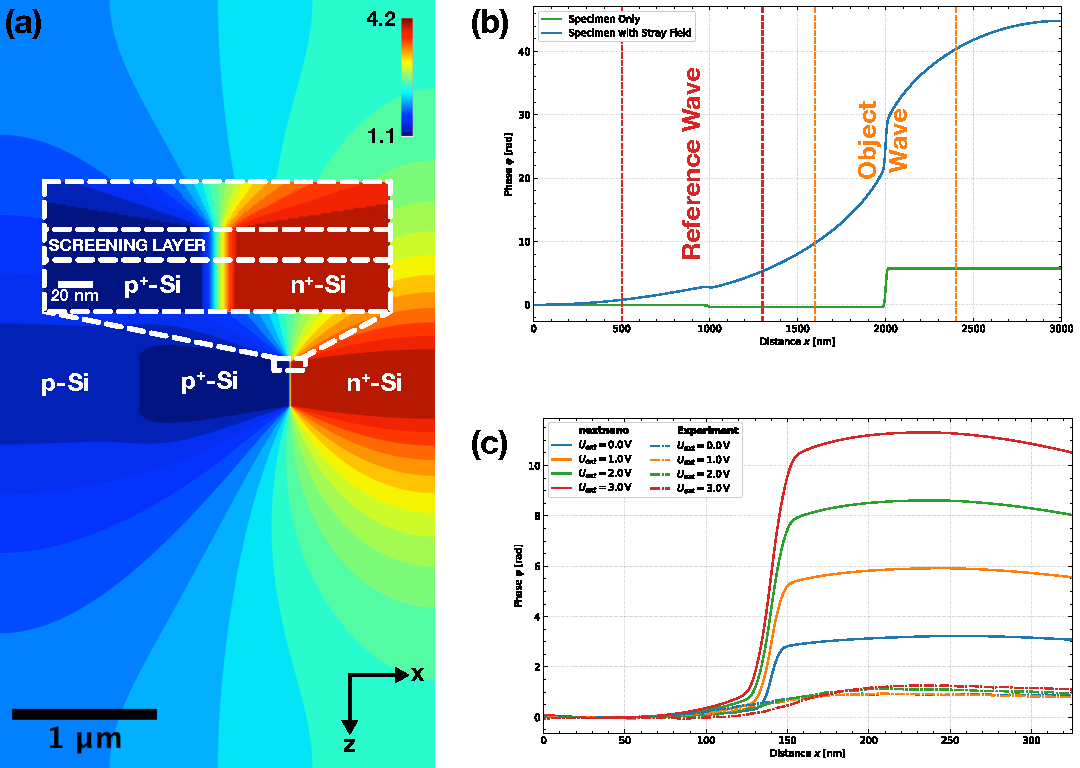
\includegraphics[width=\textwidth]{Figures/Results/pn-Junction/Simulations/pn-junction-FEM-EH-linescan-comparison.pdf}
	\caption{FEM simulation of the $p$-$p^+$-$n^+$-junction reverse biased with $U_{\mathit{ext}} = \SI{2}{\volt}$ where (a) the 2D~electrostatic potential $\phi$ yields (b) the phase $\varphi$ through projection, (c) which is compared with the above detailed experimentally acquired holograms for different applied bias voltages.}
	\label{fig:pn-junction-FEM-EH-linescan-comparison}
\end{figure}
The 2D~electrostatic potential $\phi$ obtained through this method shows, similar to the above described coplanar capacitor, that, while the contacts exhibit a constant potential in $z$-direction in agreement with the expected behavior for a reverse biased diode, the stray field extents deep into the vacuum above and below the diode\footnote{By default, \emph{nextnano} assumes von~Neumann boundary conditions.} (\cref{fig:pn-junction-FEM-EH-linescan-comparison}a). Calculating the phase $\varphi$ through a projection of the electrostatic potential (without any weighting applied to the different specimen regions), where the specimen (i.\,e.\ the region inside the doped diode) once again only contributes a small parts to the overall phase (approximately 12\% of the maximum phase shift), which is predominantly made up of the stray field contribution (\cref{fig:pn-junction-FEM-EH-linescan-comparison}b, with both phases offset to zero through subtraction by the first value). Furthermore, by centering the object wave $\varphi_{\mathit{obj}}$ around the depletion region at the $p^+$-$n^+$-interface (\cref{fig:pn-junction-FEM-EH-linescan-comparison}b, indicated by the dashed orange lines) and the reference wave $\varphi_{\mathit{ref}}$\footnote{According to \cref{ssec:FEM-simulated-potential-and-phase}, only the stray field contribution is considered for the reference wave (\cref{fig:flowchart-automatic-nextnano-post-processing}).} around a region of equal size offset $\SI{300}{\nm}$ to the left (\cref{fig:pn-junction-FEM-EH-linescan-comparison}b, indicated by the dashed red lines), comparisons to the above experimentally acquired phases are made (\cref{fig:pn-junction-FEM-EH-linescan-comparison}c).

For every externally applied reverse bias $U_{\mathit{ext}}$ ranging from $\SIrange{0.0}{3.0}{\volt}$, the simulated phases were an order of magnitude larger their phase jump and an order of magnitude smaller in their depletion region width, indicating large deviations between them. Even when taking into account the significantly smaller phase jumps, the experimentally acquired holograms do not exhibit the linear proportionality between the phase jumps and the externally applied bias voltage, suggesting an abnormal switching behavior caused by improper contacting.

The screening layer at the surface of the diode, whose thickness is characterized by the Debye length $\lambda_D$, has a negligibly small contribution to the overall phase, where $\lambda_D = \SI{18 \pm 5}{\nm}$ (\cref{fig:pn-junction-FEM-EH-linescan-comparison}a) is in the expected range for a sheet-like specimen \cite{Gurugubelli2015}. It is also worth noting that \emph{nextnano} only calculates the electrostatic potential $\phi_{\mathit{pn}}$ without considering the mean inner potential $\phi_{\mathit{MIP}}$ (\cref{eq:EH-phase-shift-specimen}), whose contribution, however, does not need to be taken into account due to the $p^+$-$n^+$-junction being a homojunction (i.\,e. $\phi_{\mathit{MIP}}$ would only add a constant phase shift).

Here, the experimentally acquired 2D~phase images were likewise modulated through the subtraction of a phase wedge (\cref{eq:holosuite-phase-wedge,eq:holosuite-phase-wedge-average-fit}), whereas the simulated phases were modulated through the subtraction of a linear fit, ranging from 10\% to 20\% and extrapolated to the entire field of view, from all values (\cref{ssec:FEM-simulated-potential-and-phase}).
\newpage
The above detailed simulations represent the electrostatic potential of a specimen that has suffered no sub-surface preparation damage. Even when accounting for the spatially widely extended stray field, which extends several $\si{\um}$ deep into the vacuum above and below the specimen, the simulated phases fail to accurately represent the experimentally obtained results, deviating by an order of magnitude in both the maximum phase shift and the depletion region width.

These observations suggest the existence of an electrically damaged crystalline layer (below the electrically inactive surface layer) resulting from Ga-induced defects during the FIB preparation stage (\cref{fig:FIB-preparation-damage-layer}), which is in agreement with previous results \cite{Twitchett2002,Beleggia2003,Cooper2006,Cooper2007,Twitchett-Harrison2007,Cooper2009,Somodi2013,Yazdi2015}.
\begin{figure}[H]
	\centering
	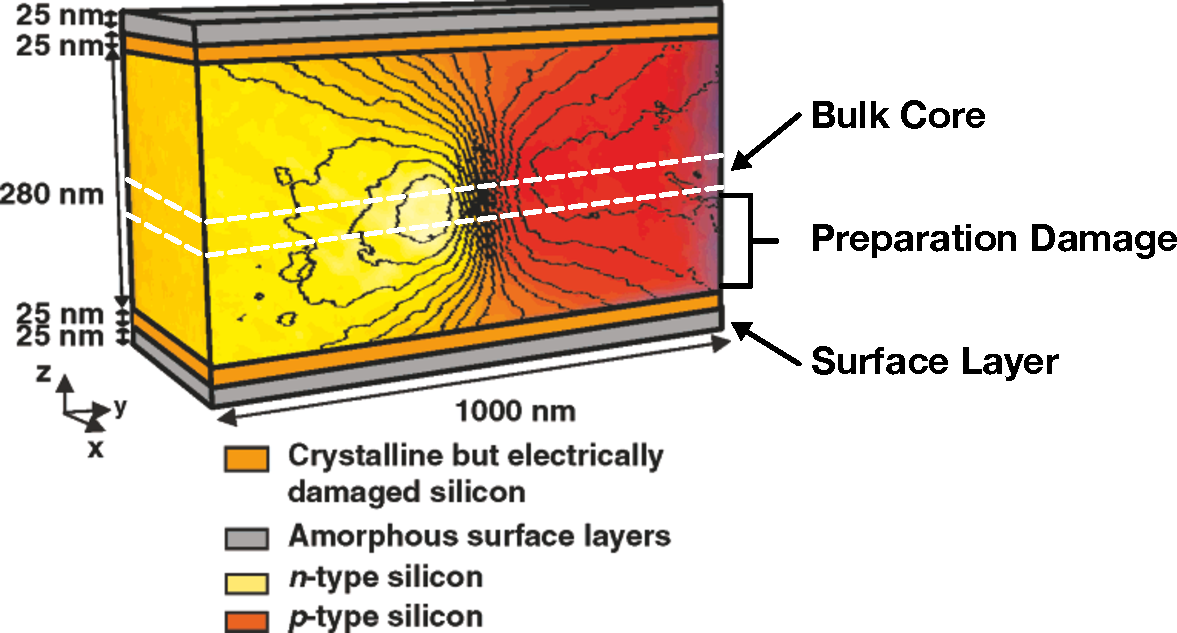
\includegraphics[width=\textwidth]{Figures/Schematics/FIB-preparation-damage-layer.pdf}
	\caption{3D~electrostatic potential obtained from the tomographic reconstruction of an electrically biased $p$-$n$-junction. Ga-induced defects caused by the FIB preparation of the specimen result in an electrically damaged crystalline layer below the electrically inactive surface layer (adapted from \cite{Twitchett-Harrison2007}).}
	\label{fig:FIB-preparation-damage-layer}
\end{figure}
Since the description of such damage effects with conventional FEM software packages proves to be impractical (as the exact distribution of the defects cannot be known), an alternative model, capable of accurately describing such real-world preparation defects (ideally with minimal prior knowledge of the specimen), is needed.
